\section{Рубежный контроль 3}

\subsection{Сформулировать определения случайной величины и функции распределения вероятностей случайной величины. Записать основные свойства функции распределения.}

Случайной величиной естественно называть числовую величину, значение которой зависит от того, какой именно \textbf{элементарный исход} произошел в результате эксперимента со случайным исходом.
Множество всех значений, которые случайная величина может принимать, называют \textbf{множеством возможных значений} этой \textbf{случайной величины.}

\textbf{Определение}

Пусть ($\Omega$, $\beta$, P) --- вероятностное пространство.

Случайной величиной называется функция $X : \Omega \rightarrow R$
Такая, что $\forall x \in \Re$ множество $(\omega : X (\omega) < x) \in \beta$.

\textbf{Определение}

Функцией распределения вероятностной случайной величины X называется отображение $F_X : R \rightarrow R$, определяется правилом $F_X(x) = P\{X < x\}$

\textbf{Свойства}

\begin{enumerate}[label=\arabic*.]
	\item $\lim\limits_{x \rightarrow -\infty}F_X(x) = 0, \lim\limits_{x \rightarrow +\infty}F_X(x) = 1$;
	\item $0 \leq F(x) \leq 1$;
	\item $F(x_1) \leq F(x_2)$, при $x_1 < x_2$ ($F_x$ --- не убывающая функция);
	\item $P\{a \leq X < b\} = F_X(b) - F_X(a)$;
	\item $\lim\limits_{x \rightarrow x_0}F_x(x) = F_X(x_0)$ --- функция распределения непрерывна слева в каждой точке $x_0$.
\end{enumerate}

\subsection{Сформулировать определение дискретной случайной величины; понятие ряда распределения.Сформулировать определение непрерывной случайной величины и функции плотности распределения вероятностей.}

\textbf{Определение}: Дискретная

Случайная величина называется дискретной, если множество ее возможных значений конечно или счетно.

Если множество значений дискретной случайной величины конечно, то закон ее распределения можно задать с использованием таблицы.
\begin{table}[ht!]
	\begin{center}
		\caption{Все воможные значения СВ X $p_i = P\{X=x_i\}, i = \overline{1,n}$}
		\label{tbl:best}
		\begin{tabular}{|c|c|c|c|c|}
			\hline
			X & $x_1$ & $x_2$ & $\dots$ & $x_n$ \\ 
			\hline
			P & $p_1$ & $p_2$ & $\dots$ & $p_n$ \\
			\hline
		\end{tabular}
	\end{center}
\end{table}

\textbf{Определения}

Таблицу \ref{tbl:best} называется рядом распределения дискретной случайной величины.

\textbf{Определение}

Случайной величиной X называется непрерывной, если $\exists f: \Re \rightarrow \Re: \forall x \in \Re$ значение $F_X(x)$ можно представить в виде:\
$F_X(x) = \int_{\infty}^{\infty} f_X(t)dt$ При этом f называется функцией плотностью распределения случайной величины X.

\subsection{Сформулировать определение непрерывной случайной величины. Записать основные свойства функции плотности распределения вероятностей непрерывной случайной величины.}

\textbf{Свойства}

\begin{enumerate}[label=\arabic*.]
	\item f(x) $\leq$ 0, $x \in \Re$;
	\item $P\{x_1 \leq X < x_2\} = \int_{x_1}^{x_2}f(x)dx$;
	\item $\int_{\infty}f(x)dx = 1$ - условие нормировки;
	\item $P\{x_0 \leq X < x_0 + \Delta x\} \eqsim f(x_0)\Delta x$, где $\Delta x$ --- мало, а f --- непрерывна а точке $x_0$;
	\item Если X --- непрерывна СВ, то для $\forall$ наперед заданной точке $x_0$ $P\{X=x_0\}=0$.
\end{enumerate}


\subsection{Сформулировать определения случайного вектора и его функции распределения вероятностей. Записать свойства функции распределения двумерного случайного вектора.}

\textbf{Определение}

n - мерным случайным вектором называется кортеж $(X_1, \dots, X_n)$, где $x_i, i=\overline{1,n}$ --- СВ, заданные на одном вероятностном пространстве.

\textbf{Определение}

Функцией распределения случайная вектора

$\overrightarrow{X} = (x_1, \dots x_n)$ называется отображение $F: \Re^n \rightarrow \Re$, определенной правилом $F(x_1, \dots, x_n) = P\{X_1 \leq x_1\ \dots, X_n < x_n\}$.

\textbf{Свойства}

\begin{enumerate}[label=\arabic*.]
	\item $0 \leq F(x_1, x_2) \leq 1$
	\item \begin{itemize}
		\item при фиксированном $x_2$ функция $F(x_1, x_2)$, как функция переменная $x_1$ является неубывающей
		\item аналогично $x_1$
	\end{itemize}
	\item $\lim\limits_{x_1 \rightarrow -\infty}F_x(x_1, x_2) = 0$, $\lim\limits_{x_2 \rightarrow -\infty}F_x(x_1, x_2) = 0$;
	\item $\lim\limits_{x_2 \rightarrow +\infty, x_1 \rightarrow +\infty}F(x_1, x_2) = 1$
	\item $\lim\limits_{x_2 \rightarrow +\infty, x_1 = const}F(x_1, x_2) = F_{X_1}(x_1)$, $\lim\limits_{x_1 \rightarrow +\infty, x_2 = const}F(x_1, x_2) = F_{X_2}(x_2)$
	\item $P\{a_1 \leq X_1\ < b_1, a_2 \leq X_2 < b_2\} = F(a_1, a_2) + F(b_1, b_2) - F(a_1, b_2) - F(b_1, a_2)$
	\item При фиксированном $x_2$ функция $F(x_1, x_2)$ как функция переменной $x_1$ является непрерывной слева во векторе. Аналогично $x_1$
\end{enumerate}

\subsection{Сформулировать определение дискретного случайного вектора; понятие таблицы распределения двумерного случайного вектора. Сформулировать определения непрерывного случайного вектора и его функции плотности распределения вероятностей.}

\textbf{Определение}

Случайный вектор $\overrightarrow{X} = (X_1, \dots, X_n)$ называется дискертным, если каждая из случайных величин $X_i, i=\overline{1,n}$ является дискретной.


\textbf{Таблица распределения}

Рассмотрим случай n=2

Пусть: 
\begin{enumerate}[label=\arabic*.]
	\item (X, Y) - двумерный вектор --- дискретный;
	\item будем считать, что X и Y принимают конечное множество значений.  
\end{enumerate}
$X \in \{x_1, \dots, x_n\}, Y \in \{y_1, \dots, y_n\}$

Это означает, что случайны вектор (X, Y) может принимать значения $(x_i, y_i)$, $i=\overline{1,m}, j=\overline{1,n}$. Закон распределения такого вектора часто задают таблицей:
 
\begin{table}[ht!]
	\begin{center}
		\caption{$p_{ij} = P\{(X, Y)=(x_i, y_j)\} = P\{\{X=x_i\} \cdot \{Y=y_j\}\} = P\{X=x_i, Y=y_j\}, $ при этом достаточно выполняется условие нормировки $\sum_{m}^{i=1}\sum_{n}^{j=1}p_{ij}=1$;}
		\label{tbl:best}
		\begin{tabular}{|c|c|c|c|c|c|c|}
			\hline
			$XY$ & $y_1$ & $\dots$ & $y_j$ & $\dots$ &  $y_n$ & $P_X$\\  \hline
			$x_1$ & $p_{11}$ & $\dots$ & $p_{1j}$ & $\dots$ &  $p_{1n}$ & $p_{x1}$\\  \hline
			$\dots$ & $\dots$ & $\dots$ & $\dots$ & $\dots$ &  $\dots$ & $\dots$\\  \hline
			$x_i$ & $p_{i1}$ & $\dots$ & $p_{ij}$ & $\dots$ &  $p_{in}$ & $p_{xi}$\\  \hline
			$\dots$ & $\dots$ & $\dots$ & $\dots$ & $\dots$ &  $\dots$ & $\dots$\\ \hline
			$x_m$ & $p_{m1}$ & $\dots$ & $p_{mj}$ & $\dots$ &  $p_{mn}$ & $p_{xm}$\\  \hline
			$p_y$ & $p_{y1}$ & $\dots$ & $p_{yj}$ & $\dots$ &  $p_{yn}$ & $1$\\  
			\hline
		\end{tabular}
	\end{center}
\end{table}

\textbf{Определение}

Случайный вектор $(X_1, \dots X_n)$ называется непрерывным, если его функцию распределения можно представить в виде: 
\begin{equation}
	F_X(x_1, \dots, x_n) = \int_{-\infty}^{x_1}dt_1\int_{-\infty}^{x_2}dt_2 \dots
	\int_{-\infty}^{xn1}dt_n.
\end{equation}

При том функция $f$ называется функцией плотности распределения вероятностей случайного вектора $(X_1, \dots X_n)$.

\subsection{Сформулировать определения непрерывного случайного вектора и его функции плотности распределения вероятностей. Записать основные свойства функции плотности распределения двумерных случайных векторов.}

\textbf{Свойства} для n = 2

\begin{enumerate}[label=\arabic*.]
	\item $f(x_1, x_2) \leq 0$;
	\item $P\{a_1 \leq X_1 \leq b_1, a_2 \leq X_2 \leq b_2\} = \int_{a_1}^{b_1}dx_1\int_{a_2}^{b_2}f(x_1, x_2)dx_2$;
	\item $\int\int\limits_{R_1} f(x_1, x_2)dx_1dx_2 = 1$;
	\item $P\{x_1 \leq X_1 < x_1 + \Delta x_1, x_2 \leq X_2 < x_2 + \Delta x_2\} \eqsim f(x_1, x_2) \Delta x_1 \Delta x_2$, если $(x_1, x_2)$ - точка непрерывности функции f;
	\item Если $(X_1, X_2)$ --- непр. случайные вектор, то для $\forall$ наперед заданного $(x_1^0, x_2^0), P\{(X_1, X_2 = (x_1^0, x_2^0))\} = 0$;
	\item $P\{(X_1, X_2) \in \DJ\} \int\int\limits_{\DJ}f(x_1, x_2)dx_1dx_2$;
	\item $\int_{\infty}^{\infty}f(x_1, x_2)dx_2 = f_{x_1}(x_1) \int_{\infty}^{\infty}f(x_1, x_2)dx_1 = f_{x_2}(x_2)$
\end{enumerate}

\subsection{Сформулировать определение независимых случайных величин. Сформулировать свойства независимых случайных величин. Сформулировать определение попарно независимых случайных величин и случайных величин, независимых в совокупности.}

\textbf{Это не надо, но мне жалко это выкидывать}

Пусть 
\begin{enumerate}
	\item (X, Y) --- дискретный случайны вектор множество значений, которого конечно;
	\item причем $X \in \{x_1, \dots x_m\} Y \in \{y_1, \dots y_n\}$;
	\item $x_1 < \dots < x_n y_1 < \dots < y_n$.
\end{enumerate}

В случае такого случайного вектора (X, Y) определение независимых случайных величин по аналогии с определением событий можно сформулировать так:

X, Y называют независимыми., если $P\{(X, Y)=(x_i, y_j)\} = P\{X=x_i\} \cdot P\{Y=y_i\}; \{P\{\{X=x_i\}\{Y=y_i\}\}\},$ $i=\overline{1,m}, j=\overline{1,n}$ 

\textbf{Это надо}

\textbf{Определение}

Случайный величины X и Y называются независимыми, если $F(x, y) = F_X(x)F_Y(y)$, где F --- совместная функция распределения случайных величин X и Y.

$F_X, F_Y$ --- маргинальная функция распределения случайных величин X и Y.

\textbf{Свойства}

\begin{enumerate}[label=\arabic*.]
	\item Случайные величины X и Y незав. $\Leftrightarrow$ для $\forall x \in \Re, \forall y \in \Re$ события $\{X<x\}$ и $\{Y < y\}$ независимы.
	\item Случайные величины X, Y независимы $\Leftrightarrow$ $\forall \forall x_1, x_2 \in \Re$ $\forall \forall y_1, y_2 \in \Re$ события $\{x_1 \leq X < x_2\}$ и $\{y_1 \leq Y < y_2\}$ независимы.
	\item Случайные величины X и Y независимы $\Leftrightarrow$ $\forall M_1$ и $\forall M_2$ события $\{X \in M_1\}$ и $\{Y \in M_2\}$ независимы, где $M_1, M_2$ --- промежутки или обозначения промежутков в $\Re$
	\item Если \begin{enumerate}[label=\arabic*]
		\item X и Y дискретная случайная величина;
		\item $X \in \{x_1, \dots, x_n\}$, $Y \in \{y_1, \dots, y_n\}$;
		\item $P\{(X, Y)=(x_i, y_j)\} = p_{ij}$, $P\{X=x_i\}=p_{xi}, P\{Y=y_i\}=p_{yi}$, $i=\overline{1,m}, j=\overline{1,n}$,
	\end{enumerate}
	то X, Y независимы $\Leftrightarrow$ $p_{ij} = p_{xi}p_{y_i}$ $i=\overline{1,m}, j=\overline{1,n}$
	\item Если X, Y непрерывные случайные величины, то X, Y независимы $\Leftrightarrow$ $f(x, y) = f_X(x)f_Y(y)$, где f --- совм. плотность распределения случайного вектора X и Y $f_X, f_Y$ --- ера плотности.
\end{enumerate}

\textbf{Определение}

Случайный величины $X_1, \dots, X_n$ заданные на одном и том же вероятностном пространстве, называют \textbf{независимыми в совокупности}, если $F(x_1, \dots, x_n) = F_{X_1}(x_1) \dot \cdot \dot F_{X_n}(x_n)$, где F --- совместная функция распределения случайных величин $X_i, \forall i,j = \overline{1,n}, i \neq j$.

\textbf{Определение}

Случайный величины $X_1, \dots, X_n$, заданные на одном и том же вероятностном пространстве, называют \textbf{независимыми в попарно}, если $x_i$ и $x_j$ независимы  для $\forall i,j = \overline{1,n}, i \neq j$.

\subsection{Понятие условного распределения. Доказать формулу для вычисления условного ряда распределения одной компоненты двумерного дискретного случайного вектора при условии, что другая компонента приняла определенное значение. Записать формулу для вычисления условной плотности распределения одной компоненты двумерного непрерывного случайного вектора при условии, что другая компонента приняла определенное значение.}


Пусть дан двумерный СВектор $(X, Y)$ и известно, что СВ $Y$ принимает значение $y$.


Пусть $(X, Y)$ – дискретный СВектор; $X \in \{x_1, \dots, x_n\}$, $Y \in \{y_1, \dots, y_n\}$ $P\{(X, Y)=(x_i, y_j)\} = p_{ij} = P\{X=x_i, Y=y_j\}$. Пусть для некоторого j $Y=y_j$; $P\{X=x_i, Y=y_j\} = \frac{P\{(X, Y)=(x_i, y_j)\}}{P\{Y=y_j\}}$ $=\frac{p_{ij}}{p_{yj}}$. Условной вероятностью того, что СВ Х примет значение $x_i$ при условии что $Y$ принимает значение $y_j$, называется число $\Pi_{ij}=\frac{p_{ij}}{p_{yj}}$; набор вероятностей $\Pi_{ij}, \forall i, j$ называется условным распределением СВ Х.

Пусть $(XY)$ --- непрерывный СВектор. Условной функцией распределения СВ Х при условии $Y = y$ называется отображение $F_X(x|Y=y) = P\{X < x|Y=y\}$ Условной плотностью распределения СВ Х при условии $Y=y$ называется функция $f_X(x|Y=y)=\frac{f(x, y)}{f_Y(y)}$, где $f(x,y)$ --- совместная плотность распределения СВектора.

\subsection{Сформулировать определение независимых случайных величин. Сформулировать критерий независимости двух случайных величин в терминах условных распределений.}

\textbf{Определение}

Случайный величины X и Y называются независимыми, если $F(x, y) = F_X(x)F_Y(y)$, где F --- совместная функция распределения случайных величин X и Y.

\textbf{Критерий}

\textbf{Критерий независимости случайных величин} $X$ и $Y$. \textit{Случайные величины} X и Y являются \textit{независимыми} $\Leftrightarrow$ условное распределение (функция распределения,
плотность распределения) случайной величины $X$ при условии $Y = y$ совпадает с безусловным распределением (функцией распределения, плотностью распределения) случайной величины X.

В частности, дискретные величины X и Y являются независимыми $\Leftrightarrow$ все условные вероятности
\begin{equation}
	\pi_{ij} = P\{X = x_i |Y = y_j\}
\end{equation}

совпадают с безусловными вероятностями 

\begin{equation}
	px_i = P\{X = x_i\}.
\end{equation}


\subsection{Понятие функции случайной величины. Указать способ построения ряда распределения функции дискретной случайной величины. Сформулировать теорему о плотности распределения функции от непрерывной случайной величины.}

Рассмотрим на \textit{вероятностном пространстве} ($\Omega$, $\beta$, P) двуменрный \textit{случайны вектор} $\overrightarrow{X} = (X_1; X_2)$ и числовую функцию $y = \phi(x_1, x_2)$ числовых аргументов $x_1, x_2$

\textbf{Определение}. Случайную величину

\begin{equation}
	\label{stroganov-pidoras}
	Y = \phi(X_1, X_2) = \phi(X_1(\omega), X_2(\omega))
\end{equation}

называют \textbf{функцией (скалярной) от двумерной случайной величины (двумерного случайного вектора)} $(X_1;X_2)$.

Ясно, что функция $Y = \phi$ от двумерной дискретной случайной величины $(X_1;X_2)$ является дискретной случайной величиной, принимающей значения $\phi (x_{1i}, x_{2j})$ с вероятностью $p_{ij} = P\{X_1 = x_{1i}, X_2 = x_{2j}\}, $ где $x_{1i}, x_{2j}$ --- значения случайных величин $X_1, X_2$ соответственно.

Чтобы построить \textbf{ряд распределения случайной величины} $Y = \phi(X_1, X_2)$, необходимо, не учитывать все те значения $\phi(x_{1i}, x_{2j})$, вероятность принять которые случайной величине Y равна нулю, а во-вторых, объединить в один столбец все одинаковые значения $\phi(x_{1i}, x_{2j})$ случайной величины Y, приписав этому столбцу суммарную вероятность.

\textbf{Теорема}

В том случае, когда $(X_1; X_2)$ --- \textit{двумерная непрерывная случайная величина с плотностью распределения} $p_{X_1, X_2}(x_1, x_2)$, функцию распределения случайной величины $Y = \phi(X_1, X_2)$ можно найти по формуле

\begin{equation}
	\label{jopa2}
	F_Y(y) = \int\int\limits_{\phi(x_1, x_2) < y} p_{X_1, X_2}(x_1, x_2)dx_1dx_2, 
\end{equation}

где область интегрирования состоит из всех значения $x_1, x_2$ для которых $\phi(x_1, x_2) < y$

\subsection{Понятие скалярной функции случайного векторного аргумента. Доказать формулу для нахождения значения функции распределения случайной величины Y, функционально зависящей от случайных величин X1 и X2 .}

\textbf{Понятие скалярной функции случайного \dots} \ref{stroganov-pidoras}

\textbf{Доказательство}

\begin{figure}[ht!]
	\centering
	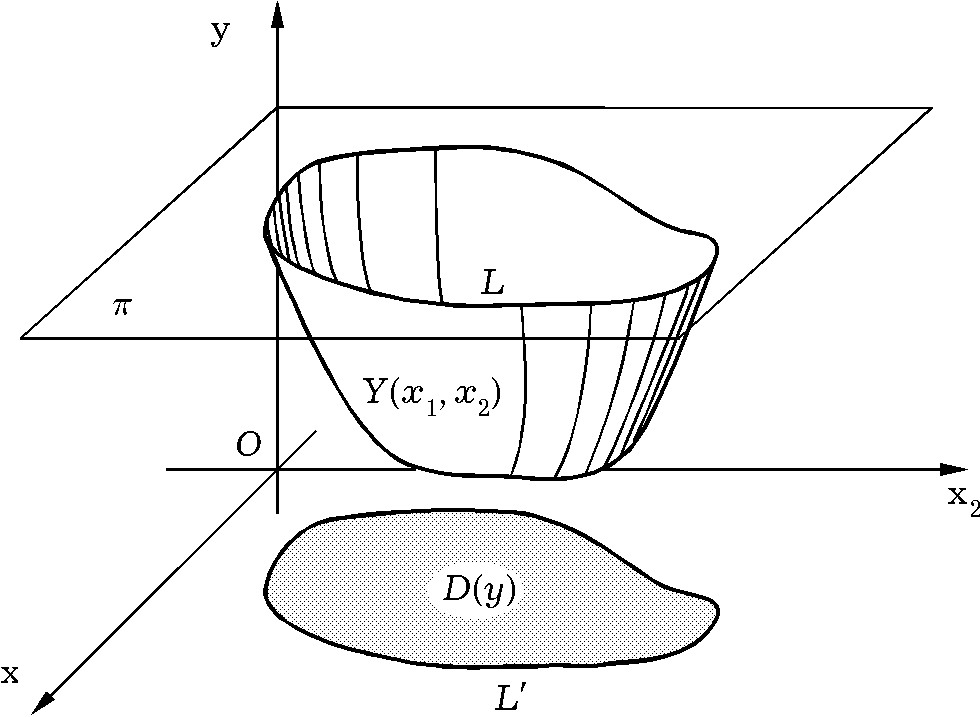
\includegraphics[width=0.6\linewidth]{assets/jopa-geom.png}
	\caption{Функция распределения}
	\label{fig:alg}
\end{figure}

Поясним геометрически вывод формулы \ref{jopa2}. Пусть поверхность, определенная функцией $y = \phi(x_1, x_2)$, имеет вид "чаши" (см. рис. \ref{fig:alg}) и y --- произвольное значение случайной величины $Y = \phi(X_1, X_2)$. Проведем плоскость $\pi$, проходящую через точку $(0, 0, y)$ и ортогональную оси $Oy$. Обозначим через L линию пересечения плоскости $\pi$ и поверхности $y = \phi(x_1;x_2); L^{`}$ --- ее проекцию на плоскость $x_1Ox_2; D(y)$ --- ту част плоскости $x_1Ox_2$, попадание в которую случайного вектора $(X_1;X_2)$ ведет к реализации \textit{события} $\{Y < y\}$. Поскольку $Y = \phi(X_1, X_2)$, то

\begin{equation}
	D(y) = \{\{x_1; x_2\} : \phi(x_1, x_2) < y\} = \{\phi(x_1, x_2) < y\}.
\end{equation}

События $\{Y < y\}$ и $\{(X_1; X_2) \in D(y)\}$ совпадают, и в соответствии со свойство 6 \textit{двумерной плотности распределения}

\begin{equation}
	P\{Y < y\} = P\{(X_1; X_2) \in D(y)\} = \int\int\limits_{\phi(x_1, x_2) < y} p_{X_1, X_2}(x_1, x_2)dx_1dx_2,.
\end{equation}

Учитывая равенство $P\{Y < y\} = 	F_Y(y)$, приходим к формуле \ref{jopa2}.

\subsection{Сформулировать и доказать теорему о формуле свертки.}

Когда $X_1, X_2$ являются \textit{независимыми случайными величинами, то есть их двумерная плотность распределения}

\begin{equation}
	p_{X_1, X_2}(x_1, x_2) = p_{X_1}(x_1)p_{X_2}(x_2)
\end{equation}

(мы ограничиваемся, здесь только случаем непрерывных случайных величин), а случайная величина Y является их суммой: $Y = X_1 + X_2$

Тогда $Y = Y(X_1, X_2)$, где $Y(x_1, x_2) = x_1 + x_2$ и согласно формуле \ref{jopa2}, находим:

\begin{align}
	\begin{split}
	F_Y(y) = \int\int\limits_{x_1 + x_2 < y} p_{X_1, X_2}(x_1, x_2)dx_1dx_2 =  \int\int\limits_{x_1 + x_2 < y} p_{X_1}(x_1) p_{X_2}(x_2)dx_1dx_2 =\\ \int\limits_{-\infty}^{+\infty} p_{X_1}(x_1)dx_1 \int\limits_{-\infty}^{y-x_1} p_{X_2}(x_2)dx_2 = \\
	\int\limits_{-\infty}^{+\infty}F_{X_2}(y-x_1)px_1(x_1)dx_1.
	\end{split}
\end{align}

Дифференцируя последнюю формулу по y под знаком интеграла, получаем (с учетом преобразования $x_1 = x$) выражение для \textit{плотности} $p_y(y)$  распределения суммы $X_1, X_2:$ 

\begin{equation}
	p_Y(y) = \int\limits_{-\infty}^{+\infty}p_{X_2}(y - x)p_{X_1}(x)dx
\end{equation}

\subsection{Сформулировать определение математического ожидания случайной величины (дискретный и непрерывный случаи). Записать формулы для вычисления математического ожидания функции от случайной величины. Сформулировать свойства математического ожидания. Механический смысл математического ожидания.}

\begin{enumerate}[label=\Roman*]
	\item X --- дискретный случайный вектор
	
	\textbf{Определение}
	
	Мат. ожидание (среднее значение) случайного вектора X M[X] = $\Sigma_ix_i p_i$, где $p_i=P\{X=x_i\}$
	
	\textbf{Замечание}
	
	\begin{itemize}
		\item Если СВ X принимает значение из счетного множества, то должен абсолютно сходится ряд $\Sigma_ix_ip_i$ сходится $\Sigma|{x_i}|p_i$. Если ряд расходится M[X] не существует.
		\item механический смысл M[X]--- центр масс. 
	\end{itemize}

	\item X --- непрерывная случайная величина f(x) --- плотности распределения.
	
	\textbf{Определение}
	
	$M[X] = \int\limits_{-\infty}^{+\infty} x \cdot f(x)dx$
	\begin{itemize}
		\item $M[X] = \int\limits_{-\infty}^{+\infty} |x| \cdot f(x)dx < \infty$. Если инт. расходится M[X] не существует.
		\item бесконечный стержень Масса (1 кг) распр. вдоль стержня вдоль по закону f(x) M[X] = m --- координаты центра масс стержня. 
	\end{itemize}
\end{enumerate}

\textbf{Формула для вычисления мат. ожидания функции от случайной величины}

X случайная величина $\phi \Re \rightarrow \Re$ 

$M[\phi(X)] = \Sigma_i\phi(x_i)p_i$, если X --- дискретная сл. вел.

$M[\phi(X)] = \int\limits_{-\infty}^{+\infty} \phi(x) \cdot f(x)dx$, если X --- непрерывная случайная величина, f(x) --- плотность.

\subsubsection*{Свойства математического ожидания}

\begin{enumerate}
	\item Если $P\{X = x_{0}\} = 1$;
	\item $M[aX + b] = a \cdot MX + b$;
	\item $M[X_{1} + X_{2}] = MX_{1} + MX_{2}$;
	\item Если $X_{1}, X_{2}$ --- независимы, то $M[X_{1}X_{2}] = (MX_{1})(MX_{2})$.
\end{enumerate}

\subsection{Сформулировать определение дисперсии случайной величины. Записать формулы для вычисления дисперсии в дискретном и непрерывном случае. Сформулировать свойства дисперсии. Механический смысл дисперсии.}

\textbf{Дисперсией} случайной величины $X$ называют число

\begin{equation}
	D[X] = M[(X - m)^{2}],
\end{equation}
где $m = MX$.

\subsubsection*{В случае дискретной случайной величины}

\begin{equation}
	D[X] = \sum_{i}(x_{i} - m)^{2}p_{i},
\end{equation}
где $p_{i} = P\{X = x_{i}\}$.

\subsubsection*{В случае непрерывной случайной величины}

\begin{equation}
	D[X] = \int_{-\infty}^{\infty}(x - m)^{2}f(x)\,dx
\end{equation}

\subsubsection*{Свойства дисперсии}

\begin{enumerate}
	\item $DX \geqslant 0$;
	\item Если $P\{X = x_{0}\} = 1$, то $DX = 0$;
	\item $D[aX + b] = a^{2}DX$;
	\item $D[X] = M[X^{2}] - (MX)^{2}$;
	\item Если $X_{1}, X_{2}$ --- независимы, то $D[X_{1} + X_{2}] = DX_{1} + DX_{2}$.
\end{enumerate}

\subsubsection*{Механический смысл}

Дисперсия случайной величины характеризует разброс значений этой случай ной величины относительно математического ожидания. Чем больше дисперсия, тем больше разброс значений.

С точки зрения механики дисперсия --- момент инерции вероятностной массы относительно математического ожидания.

\subsection{Сформулировать определения начального и центрального моментов случайной величины. Математическое ожидание и дисперсия как моменты. Сформулировать определение квантили и медианы случайной величины.}

Пусть $X$ --- случайная величина.

\textbf{Моментом $k$-ого порядка ($k$-ым случайным моментом)} случайной величины $X$ называется число

\begin{equation}
	m_{k} = M[X^{k}]
\end{equation}

\textbf{Центральным моментом $k$-ого порядка} случайной величины $X$ называется число

\begin{equation}
	\dot m_{k} = M[(X - m)^{k}],
\end{equation}
где $m = MX$.

\subsubsection*{Мат. ожидание и дисперсия как моменты}

\textbf{Мат. ожидание} --- $m_{0} = MX$.

\textbf{Дисперсия} --- $\dot m_{2} = DX$.

\subsubsection*{Определение квантили и медианы}

Пусть

\begin{enumerate}
	\item $X$ --- случайная величина;
	\item $\alpha \in (0, 1)$.
\end{enumerate}

\textbf{Квантилью} уровня $\alpha$ ($\alpha$-квантилью) случайной величины $X$ называется $q_{\alpha}$ такое, что

\begin{equation}
	P\{X < q_{\alpha}\} \leqslant \alpha, P \{X > q_{\alpha}\} \leqslant 1.
\end{equation}

\textbf{Медианой} случайной величины $X$ называют ее квантиль уровня $1/2$.

\subsection{Сформулировать определение ковариации случайных величин. Записать формулы для вычисления ковариации в дискретном и непрерывном случаях. Сформулировать свойства ковариации.}

\textbf{Ковариация} --- характеристика случайного вектора.

Пусть $(X, Y)$ --- двумерный случайный вектор.

\textbf{Ковариацией} случайных величин $X$ и $Y$ называется число

\begin{equation}
	cov(X, Y) = M[(X - m_{X})(Y - m_{Y})],
\end{equation}

где $m_{X} = MX, m_{Y} = MY$.

\subsubsection*{В случае дискретного случайного вектора}

\begin{equation}
	cov(X, Y) =  \sum_{i}^{} \sum_{j}^{} (x_{i} - m_{X})(y_{j} - m_{Y})p_{ij},
\end{equation}

где $p_{ij} = P\{(X< Y) = (x_{i}, y_{j})\}$.

\subsubsection*{В случае непрерывного случайного вектора}

\begin{equation}
	cov(X, Y) = \int \int_{R^{2}}^{} (x - m_{X})(y - m_{Y})f(x, y)\,dx\,dy,
\end{equation}

где $f$ --- совместная плотность величин $X$ и $Y$.

\subsubsection*{Свойства ковариации}

\begin{enumerate}
	\item $D(X, Y) = DX + DY + 2cov(X, Y)$;
	\item $cov(X, X) = DX$;
	\item Если $X, Y$ --- независимые, то $cov(X, Y) = 0$;
	\item $cov(a_{1}X + b_{1}, a_{2}Y + b_{2}) = a_{1}a_{2}cov(X, Y)$;
	\item $|cov(X, Y)| \leqslant \sqrt[]{DX \cdot DY}$, причем $|cov(X, Y)| = \sqrt[]{DX \cdot DY} \iff \exists \exists a, b \in \Re, Y = aX + b$ (т.~е. $X$ и $Y$ связаны линейной зависимостью);
	\item $cov(X, Y) = M[XY] - (MX)(MY)$.
\end{enumerate}